\chapter{Introduction}
So it begins.The journey to a destination which will never be reached. The
journey to perfection! The journey to perfect programs. I have read somewhere
that a perfect program is one from which nothing can be deleted. Well, the fun
is not in the destination but in journey. The process of learning is fun. And I
will share this fun with you. Of all popular mainstream languages C, and Lisp
are two oldest but we cannot really say that Lisp is really popular. It has a
niche area and it is there for that. So let me redefine my statement. Of all
general-purpose popular programming language C is the oldest. So what makes C
so special that it is still out there. Well, C and Unix were born almost
together in early 1970s. Then Unix was ported in C and the notion that
operating systems can be only written in assembly language, because it has to
do time critical things, was destroyed. After that Unix became very
popular. Then when C++ was not yet there Windows was written in C and more and
more programs were written in C. It might have been the case that Microsoft and
Apple would have written their OS in C++ had it been there. So, essentially
what happened that there is a lot of code base which is there in C. Also, C++'s
backward compatibility is one of the reasons why C++ is so popular. When C was
invented there was no structured programming language and code was mostly
written in assembly. With C it gave the power of assembly and benefits of
structured language like code reuse, modularity, and portability among
others. Because of these reasons C became immensely popular and is still
popular.

C is simple, small, succinct. It may be dirty but is quick. It may have its
quirks but it is a success. C is really so simple yet so deceptive. It will
take one years of programming to really thoroughly understand it. Note that
this book will make heavy use of C99 specification. It will contain almost a
copy of n1124.pdf which I have.

Following is a video which I have created and is about introcution to
programming. I talk a bit about C++ in it:
\url{http://www.youtube.com/watch?feature=player\_embedded\&v=UIIrDcYSrI0}

In this video I specifically talk about C99:
\url{http://www.youtube.com/watch?feature=player\_embedded\&v=y8PSO45Krfk}

\section{Why C?}
Because it is the most common denominator. Any language be it C++, Java, Perl,
Python etc have got bindings in C. Whenever you are willing to extend these
languages you need to know C. Also, if by any chance you are going towards
system programming you need to C. C is everywhere. There is no escape from
learning it; it does not matter whether you like it or not.

There is one more important point worth noting here is that C++ is far more
complex compared to C. Also, the runtime calculations of C++ make it slightly
slower than C. The library of C is much smaller than C. Therefore wherever
there is a memory constraint or extreme high performance is needed C is
preferred. The simple syntax of C means its code is very verbose for programmer
in the sense that if you read code then you can very easily see what
instructions the code is going to translate into.

It is very easy to write interfaces to other languages because other languages
expose there objects in terms of C structures not the other way around. The
reason for this is huge popularity of C and large code base perhaps.

One more important feature is portability. Note that if you want your program
to have high degree of portability then you should not use C99 features but
rather ANSI C because ANSI C compilers are available on most platforms. Even
though Java claims to be portable or other interpreted languages they are
limited by the fact that the interpreters or VMs(JVM in case of Java) is not
available on all the platforms. Therefore, C is the MOST portable language. :-)

\section{History}
C was formally delivered to this world in 1972 and conceived by Dennis
MacAlistair Ritchie in 1968. What happened was there was a project for
development of a text processor and GE-645 was bought by AT\&T Bell Labs. At
that time Ken Thompson had developed a game called ``Space Travel''. Then they
had another machine PDP-11. Before that they had PDP-7. Now all the time the
code for ``Space Travel'' had to be rewritten and also the Unix had to be
ported. So when C was invented it was used to write Unix code in C. And then
``Space Travel''. I do not know what was the real motivation the language, the
OS or the game. But such is the story. Also, I have not studied much in this 
about the exact events. In 1972 C was formally announced. C takes its features
from BCPL a language by Martin Richard and B by Ken Thompson. AT\&T Bells labs
gave Unix and a C compiler to many universities at a normal fees and it grew
with leaps and bounds from there and became a ubiquitous language. For many
years ``The C Programming Language'' served as a reference of C. Later it was
standardized by ANSI and then by ISO standards. A very detailed history of C
programming language can be found at
\url{http://cm.bell-labs.com/cm/cs/who/dmr/chist.html} which has been described
by Dennis Ritchie himself.
\index{Dennis Ritchie}
\index{Ken Thompson}

\section{Comparison with Other Languages}
C is a structured, statically typed, somewhat low-level, high-performance
compiled language. It does not support object-oriented programming like most
modern programming including C++, Java, Perl, Python, Ruby etc. However, that
does not mean you cannot do object-oriented programming in C. It is just that C
does not have support at the language level and it is painful to do so. C is
low level because it allows you to handle memory contents directly. You have
something called void which is raw representation of memory content. C also
does not support functional or generic programming but again it is possible to
do so with painful hacks. One of the coveted features is C programs deliver
very high performance if written correctly as it does not have runtime
penalties of virtual functions of OOP (object-oriented programming) languages.

\section{How to learn programming?}
Programming is exactly like Mathematics. As in Mathematics you need to read
theory, understand solved problems and then solve more and more problems by
yourself. If you cannot solve ask your teacher. Similarly, in programming you
need to read about language, try examples given, read code written by others
and then develop your own code. If you get stuck there are umpteen number of
tutorials, mailing lists and groups to help you. I recommend comp.lang.c user
group for C programming. Its interface is at
\url{http://groups.google.com/group/comp.lang.c/}. You should join it and
participate there. \url{http://www.stackoverflow.com/} is also a very good
forum to ask questions about programming in general. You can also come at my
website \url{http://qa.libreprogramming.org} or
\url{http://kunjika.libreprogramming.org} and ask questions or have a
discussion. Please note that later on \textit{qa} will be merged into
\textit{kunjika}.

\section{What is a computer Program?}
Since this book is written for even beginner please allow me to start from
beginning. As the reader may know a computer consists of many components and
one of the most or rather most important part is processor often named as CPU
(central processing unit). The logic gates in CPUs are formed and instructions
like ADD (addition), SUB (subtraction), MUL (multiplication), DIV (division)
etc are implemented in hardware of CPU. When we write a program say C program
the instructions given in our program is translated to a format which operating
system can understand. In our case that is GNU/Linux this executable format is
known as ELF (executable and linkable format). For the curious you can read
http://en.wikipedia.org/wiki/Executable\_and\_Linkable\_Format and there are
lots of specification for different CPUs. Then operating system interprets
these files and ask CPU to perform action. So a C program does not directly
talk to processor but it rather talks to operating system or kernel of the
operating system and in turn the operating system or kernel provides services
to your program. There is a typical life cycle in development of a C
program. First you, the programmer, uses a text editor like \texttt{Emacs} to
enter the program then you use a compiler like \texttt{gcc} to compile the
program. Then you may get warnings and errors either from prepreocessor,
compiler or linker all of which are wrapped by \texttt{gcc} in one step. Now
there can be error in your compilation command, which, you used to compile the
program or the program itself. If the error is in command then we need to fix
the command or if the error is in program then we need to fix the program and
compile it again. However, only successful compilation does not guarantee that
program is working. It must run well also. If it does not run well then
somewhere in code things are wrong and then we need to either examine the
source code or debug it using a debugger like \texttt{gdb}. Given below is the
complete cycle of what we do in development of a program as a diagram for quick
understanding.

\begin{figure}[t!]
\begin{center}
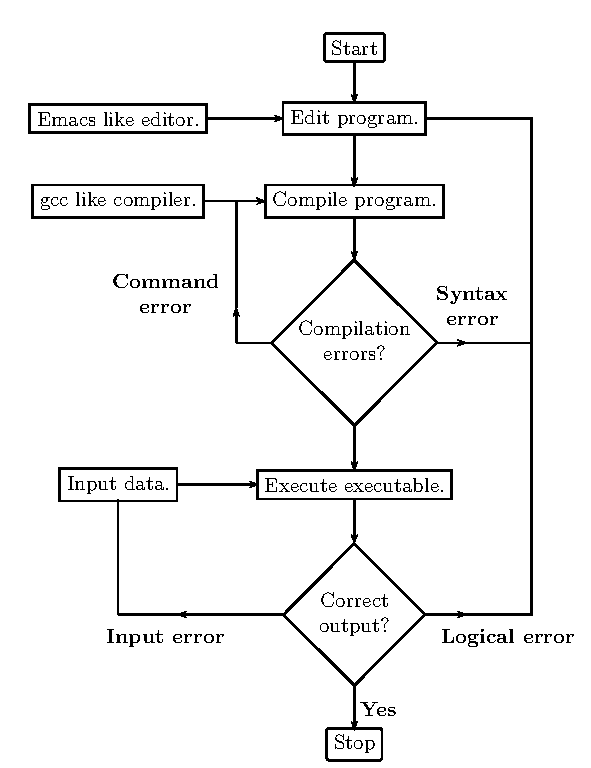
\includegraphics{figs/flowchart-fig1.pdf}
\end{center}
\caption{Life cycle of development of a program}
\end{figure}

\section{Attributes of a Program}
You may be wondering so that is very easy. You just learn programming in C and
start hacking on keyboard to produce software. Well, that is partially true but
a program has several desired attributes which you must consider. Any program
cannot be considered a good program unless it satisfies following requirements
or possess following attributes (Note: These are generic attributes and not
specific to C programming language):
\index{program!attributes}
\begin{enumerate}
\item \textbf{Correctness:}  Correctness means that a program satisfies its
  requirement specification. It means that for a specified input the specified
  output should be produced. This particular attribute is of most
  significance. It does not matter whether other attributes are present or not
  but this one is a must. If a program behavior is not correct then it is of no
  use.
\item \textbf{Efficiency:} Efficiency is second to correctness only. Say you
  are developing a text editor and you take 5 seconds to load a 10KB text file
  then by no means you can persuade a user to use you text editor. A
  program/software must be as efficient as possible. Sometimes it clashes with
  other attributes and also depend on the problem domain that how strict are
  the requirements.
\item \textbf{Security:} A very highly desirable feature in programs which deal
  with more than one computer and also for desktop applications. It is very bad
  if someone can take advantage of buffer overflow, stack overflow, integer
  overflow etc. in your program and you must guard against these at all
  times. Note that to provide security you must put extra checks which will go
  against efficiency.
\item \textbf{Robustness:} Sometimes users will not give correct inputs. For
  example they may enter a character when an integer is asked for or they can
  give input beyond range. In such cases you must handle the erroneous
  input. This is just one example. Sometimes your memory allocation may
  fail. The rule is program defensively. All such input validations and checks
  on memory do take a toll on our second attribute but that does not mean that
  we can neglect it.
\item \textbf{Maintainaibility:} Even a one line program has to be maintained
  if it is worth it! Typically the life of a program far exceeds the
  development time. In almost all the cases the original programmer is not
  maintainer. Because of these reasons you must strive for maintainability. You
  should follow some coding standards like I highly recommend
  \url{http://www.gnu.org/prep/standards/}. Clear documentation is one of the
  prerequisites of maintainability.
\item \textbf{Extensibility:} Let us take our example of text editor and say
  our editor is complete. Now someone else would like to provide a plugin which
  will enable syntax highlighting and project management for this editor. So,
  in order to do so you can choose a plugin-based extensible architecture or
  you can allow them to extend the editor using scripting languages like Guile,
  Python, Lua etc.This features allows user to collaborate and make your
  program better. Remember the rule is the more the merrier here.
\item \textbf{Portability:} It is an elusive and painful but a goal which all
  software desire. Let us say we write our text editor GUI using something like
  Xlib directly then we will have to port the entire GUI for other non X-based
  OSes. So we can choose some cross-platform GUI libraries like GTK+, Qt,
  WxWidgets etc. Even then when system calls come in your software you can do
  not much but either write wrappers and do conditional compilation.
\end{enumerate}

\section{Tools of the Trade}
I am going to use \texttt{gcc} as compiler, \texttt{Emacs} as my editor with
\texttt{CEDET, ECB} and \texttt{Flymake}. For debugging we will debug in Emacs
itself.For dynamic memory checking, heap corruption, cache corruption etc I am
going to show you how to use \texttt{valgrind}. For profiling \texttt{gprof}
and for code coverage \texttt{gcov}. Note that you can 
use gcc for compiling programs. Most of the systems come with \texttt{gcc}. For
compiling programs I will use \texttt{GNU Make} though in the beginning I will
show you how to compile on command line. Let us begin with Emacs configuration
file \texttt{.emacs}. Given below is an excerpt of my \texttt{.emacs}:

\begin{minted}{common-lisp}
(custom-set-variables
;; custom-set-variables was added by Custom.
;; If you edit it by hand, you could mess it up, so be careful.
;; Your init file should contain only one such instance.
;; If there is more than one, they won't work right.
'(column-number-mode t)
'(cua-mode t nil (cua-base))
'(ecb-layout-name "leftright2")
'(ecb-options-version "2.40")
'(ecb-windows-height 0.2)
'(ecb-windows-width 0.2)
'(make-backup-files nil)
'(scroll-bar-mode (quote right)))
(custom-set-faces
;; custom-set-faces was added by Custom.
;; If you edit it by hand, you could mess it up, so be careful.
;; Your init file should contain only one such instance.
;; If there is more than one, they won't work right.
'(default ((t (:inherit nil :stipple nil :background "#ffffff" :foreground
"#221f1e" :inverse-video nil :box nil :strike-through nil :overline nil
:underline nil :slant normal :weight normal :height 98 :width
semi-condensed :foundry "misc" :family "fixed")))))
(require 'cedet)
(require 'semantic/analyze)
(provide 'semantic-analyze)
(provide 'semantic-ctxt)
(provide 'semanticdb)
(provide 'semanticdb-find)
(provide 'semanticdb-mode)
(provide 'semantic-load)
(load "~/.emacs.d/flymake.el")
(add-to-list 'load-path "~/.emacs.d/ecb-snap")

(require 'ecb)
(require 'ecb-autoloads)
(load "~/.emacs.d/rfringe.el")
(require 'rfringe)
(when (load "flymake" t)
(defun flymake-pylint-init ()
    (let* ((temp-file (flymake-init-create-temp-buffer-copy
    'flymake-create-temp-inplace))
    (local-file (file-relative-name
    temp-file
    (file-name-directory buffer-file-name))))
    (list "epylint" (list local-file))))

(add-to-list 'flymake-allowed-file-name-masks
    '("\.py\'" flymake-pylint-init)))
    (load-file "/usr/share/git-core/emacs/git.el")
    (".+\.c$" flymake-simple-make-init flymake-simple-cleanup
    flymake-get-real-file-name)
    (setq TeX-auto-save t)
    (setq TeX-parse-self t)
    (setq-default TeX-master nil)
    (load "auctex.el" nil t t)
    (load "preview-latex.el" nil t t)
\end{minted}

At this moment do not worry much about this. I will give a more formal
introduction to \texttt{Emacs} in its own section in tools chapter.
Just that you will need to install \texttt{flymake-mode} for which you can
consult the documentation or you can read about it at
\url{http://www.emacswiki.org/emacs/FlyMake}.

\textbf{Advice:} You can also watch a video which I have prepared and which can
serve as an introduction to Emacs and CMake at
\url{http://www.youtube.com/watch?feature=player_embedded&v=4K9C83ZNNAg} but
then it involves another build system CMake which I believe is best left for
later when you are done with the book.

Once you have got \texttt{flymake-mode} installed you can type \texttt{M-x
  flymake-mode} in any C source file to enable or disble it in
cycle. \texttt{M} stands for \texttt{Meta} key which is usually \texttt{Esc} or
\texttt{Alt} key on your keyboard. Now let us just put following in a file
called Makefile in the same directory where you intend to keep your source
files:

\begin{minted}{makefile}
check-syntax:
    gcc -o nul -Wall -S $(CHK_SOURCES)
\end{minted}


Note that the leading whitespace on second line is a \texttt{TAB} character not
spacebar whitespace. Then just copy paste the following program in
\texttt{Emacs}:

\begin{minted}{c}
//Note:This listing will not compile. It has errors.
#include <stdio.h

int main()
{
  return 0
}
\end{minted}

If you do all steps correctly you should see something like: Note the pink
background. If you move your mouse there then you will see the error/diagnostic
messages from the compiler. I recommend you to read Emacs tutorial and
man pages of Clang compiler. Note that you can modify Makefile but this
particular content must remain unchanged. It is the enabler for Flymake. The
screenshot is given below:

\begin{figure}[t!]
\begin{center}
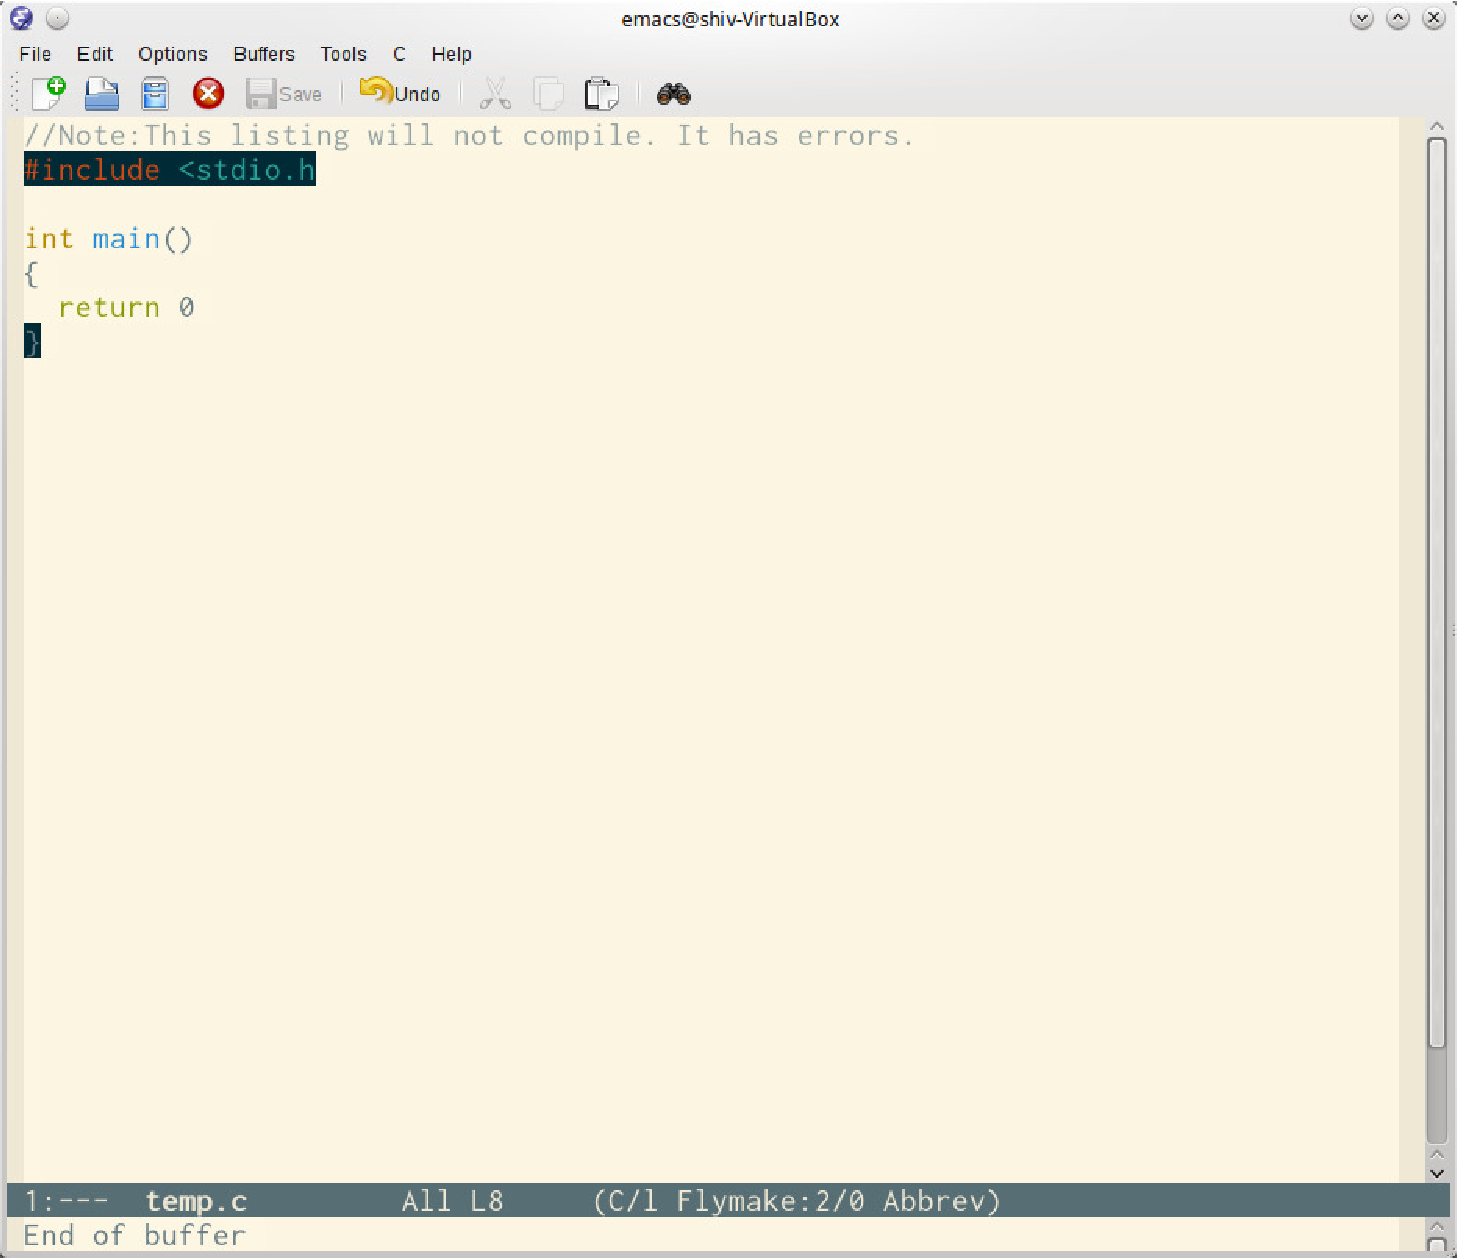
\includegraphics[width=4in]{figs/flymake.pdf}
\end{center}
\caption{Flymake with Emacs}
\end{figure}

Move your mouse over black lines to see the error.

\section{Bits and Bytes}
\index{bit}
\index{byte}
The smallest unit a computer can understand is called a bit. The term bit 
was coined by John W. Tukey who had also coined ther term software. ``bit'' 
is a contraction for binary digit. His 1958 paper ``The Teaching of Concrete 
Mathematics'' contains the first usage of the word softwrare. The values for a
\index{John Tukey}
bit is either 0 or 1. Consider a voltage. It can be 0V or 1.5V or whatever the
core CPU voltage is. CPU does not understand numbers but voltages :-). You
cannot expect an electronics hardware to understand the same semantics of 0 and
1 which we know. 0 and 1 are abstraction of CPUs voltages in programming. Four
bits form a nibble and eight a byte. A byte is the area of memory which
can be addressed by CPU and its content manipulated. To address a memory a CPU
has say 4 or 8 or up to 256 pins. For example, in a common 32-bit CPU there are
32 pins whose voltages may represent 0 or 1. Consider all pins are low i.e. 0
then the memory location pointed to is 00000000000000000000000000000000 i.e. a
8 bit memory at location 0 can be accessed. This memory is also called primary
memory or RAM (Random Access Memory). So computing this way we can see that a
32-bit processor can access $2^{32}$ bytes or 4,294,967,296 bytes. You can
arrive at this number by 4*1024*1024*1024. This is equivalent to 4GB of
RAM. However, modern Intel processors have 36 physical pins to address up to
64GB of memory.

Since a byte has 8 bits, its value may range from 0 to 255 as $2^8$ is 256. For
unsigned data type this will be the range. When all bits are 0 value is zero
and when all are high it is 255. Computers use two's complement form to
represent binary number. So if these 8-bits represent signed number the range
will be from $-2^7$ to $2^7-1$ that is -128 to 127. As you will see later at
lowest levels C allows you to access even one bit using something called
bit-fields. You should read about two's complement form at
\url{http://en.wikipedia.org/wiki/Two's\_complement} in detail. However, I will
be treating number systems in the appendices.

\section{Compiling and Executing}
\index{program!compilation}
\index{program!execution}
To compile and execute a program create a new file, edit it and save it. The
extension of file should be \texttt{*.c}. For example,
\texttt{myprogram.c}. After that you can give this command at terminal. Here is
the corrected code.

\begin{minted}{c}
#include <stdio.h>

int main()
{
  return 0;
}
\end{minted}

Execute the following command on your command prompt:

\begin{verbatim}
$clang nothing.c -o nothing
\end{verbatim}
Here \texttt{nothing.c} is the name of the file with which it was saved.

Then you will see a file named my program is created by compiler if no errors
were there in your program. In case of errors, like we had in one shown to you
they have to be resolved first. Executable \texttt{nothing} is produced then
you can execute it like

\begin{verbatim}
$./nothing
\end{verbatim}

Note that in both the commands \texttt{\$} is not part of command but it is
prompt. For you it may be \texttt{\%} or \texttt{\#} or something fancier
(depends on the imagination of your system administrator). To execute this
command your working directory must be same as the directory your program is
in. Also, note that on some systems \texttt{TAB} auto completes filename so do
not do the following by accident:

\color{nicered}
\begin{verbatim}
$clang nothing.c -o nothing.c
\end{verbatim}
\color{black}
This will overwrite your \texttt{nothing.c} by the result of compilation binary
with the same name \texttt{nothing.c}. Let us see how to compile this program
using a Makefile. Edit your \texttt{Makefile} like this:

\begin{minted}{makefile}
#sample Makefile
check-syntax:
    clang -o nul -Wall -S $(CHK_SOURCES)

nothing:nothing.c
    clang -Wall -std=c99 -pedantic nothing.c -o nothing
\end{minted}

Now from do this from menu. \texttt{Tools->compile} As the command issue
\texttt{make -k test}. Another way to do the same using keyboard only is type
\texttt{M-x compile} and repeat \texttt{make -k test} as previous time. Your
code will be compiled. Makefiles are better than executing commands 
repeatedly again and again however you must know underlying commands. I will
discuss the compiler options as appropriate. \texttt{-Wall} will enable all the
warnings from \texttt{gcc}, \texttt{-std=c99} enables new features of C99
standard and \texttt{-pedantic} ensures specification conformance. 

So let us get started with basics of C.